\documentclass[11pt,a4paper]{article}
\usepackage[T1]{fontenc}
\usepackage[utf8]{inputenc}
\usepackage{lmodern}
\usepackage{amsmath}
\usepackage{graphicx}
\usepackage[margin=22mm]{geometry}
\usepackage{booktabs,longtable,array}
\usepackage{xcolor}
\usepackage{listings}
\usepackage[hidelinks]{hyperref}

\lstset{basicstyle=\ttfamily\small, backgroundcolor=\color{black!4}, frame=single,
        rulecolor=\color{black!25}, columns=fullflexible, breaklines=true}
\newcommand{\cmd}[1]{\texttt{#1}}
\newcolumntype{L}[1]{>{\raggedright\arraybackslash}p{#1}}

\title{\texttt{gen\_hull.py}\\[1ex]\large Parametric motor-yacht hull with bulbous bow --- User manual}
\author{}
\date{November 2026}

\begin{document}
\sloppy
\maketitle
\tableofcontents
\bigskip

%=====================================================================
\section{Overview}
\cmd{gen\_hull.py} generates the hull surface of a motor yacht, $L = 20$--$50$\,m, with a
classical bulbous bow, from 33 shape parameters and one fixed datum, the displaced volume.
It writes:
\begin{itemize}
\item a structured surface grid (PLOT3D) for CFD codes;
\item the corresponding B-spline description (degree and knot vectors);
\item a STEP file, a closed solid by default;
\item a file with hydrostatics, form coefficients, Kracht's bulb parameters~\cite{kracht1978},
  stability quantities and validity checks.
\end{itemize}

Every combination of parameters inside the bounds of Section~\ref{sec:params} produces a
valid, fair hull, so the parameters can be varied freely and systematically. Several parameters
are therefore \emph{relative} (0--1): they place a quantity within its admissible range, which
depends on the other parameters, instead of prescribing an absolute value.

\begin{figure}[h]
\centering
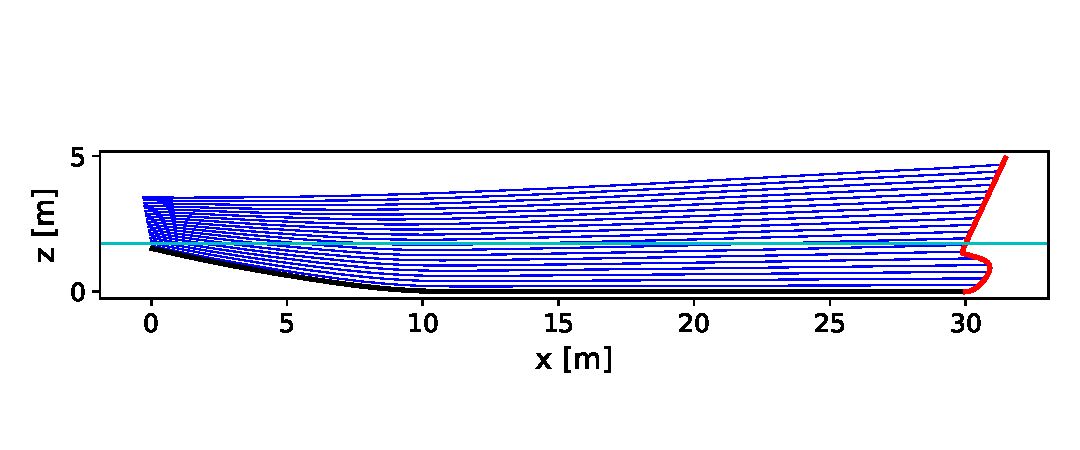
\includegraphics[width=0.9\textwidth]{figures/profile.pdf}\\
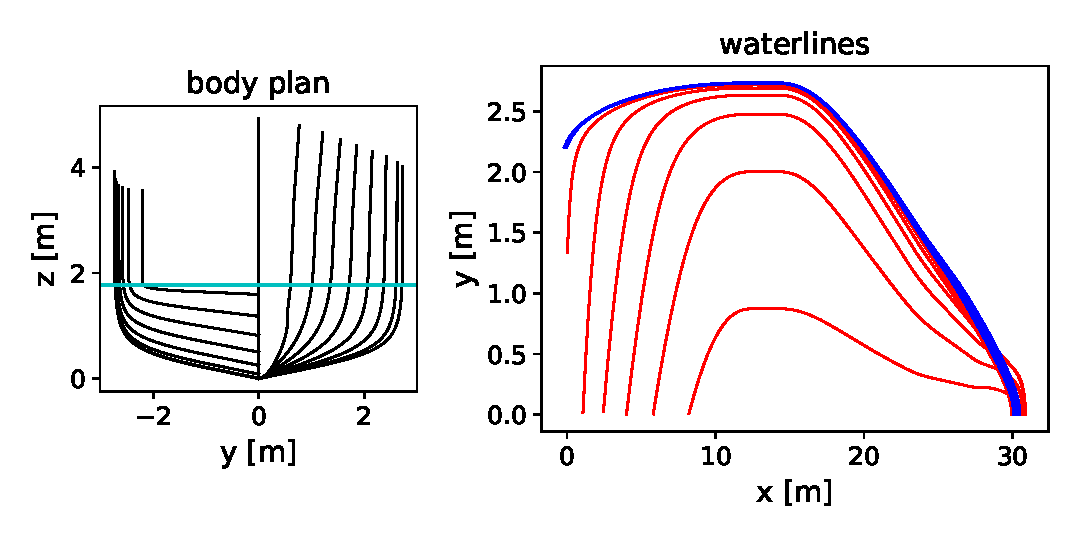
\includegraphics[width=0.9\textwidth]{figures/lines.pdf}
\caption{Default 30\,m hull: profile, body plan and waterlines.}
\end{figure}

%=====================================================================
\section{Requirements and files}
\paragraph{Requirements.} Python~3 with \cmd{numpy} and \cmd{scipy}; \cmd{matplotlib} only for
the optional 3D window and the plotting scripts. The script is a single file and needs no
installation.

\paragraph{Files.}
\begin{longtable}{L{4.9cm}L{10.4cm}}
\toprule
File & Content \\ \midrule
\cmd{gen\_hull.py} & the generator \\
\cmd{hull\_params.dat} & input parameters, one per line: \cmd{value = name} \\
\bottomrule
\end{longtable}

%=====================================================================
\section{Quick start}
\begin{lstlisting}
python3 gen_hull.py --no-plot --ni=96 --nj=32
\end{lstlisting}
This reads \cmd{hull\_params.dat} and writes \cmd{hull\_grid.p3d}, \cmd{hull\_nurbs.dat},
\cmd{hull.step} and \cmd{hull\_hydro.dat}. The last line printed reports volume, LCB, wetted
surface, LWL and whether the variant is valid (\cmd{VALID} / \cmd{NOT VALID}).
A run takes about 5\,s.

To change the hull, edit \cmd{hull\_params.dat} (or pass another file with \cmd{--params}).

%=====================================================================
\section{Command-line options}
\begin{longtable}{L{4.3cm}L{2.9cm}L{8.1cm}}
\toprule
Option & Default & Meaning \\ \midrule
\cmd{--params FILE} & \cmd{hull\_params.dat} & input parameter file \\
\cmd{--output FILE} & \cmd{hull\_grid.p3d} & PLOT3D grid \\
\cmd{--nurbs FILE} & \cmd{hull\_nurbs.dat} & B-spline degree and knots \\
\cmd{--step FILE} & \cmd{hull.step} & STEP file \\
\cmd{--hydro FILE} & \cmd{hull\_hydro.dat} & hydrostatics and checks \\
\cmd{--ni N}, \cmd{--nj N} & 32, 15 & grid size: $i$ along the hull, $j$ along the sections \\
\cmd{--degree P} & 3 & B-spline degree in both directions \\
\cmd{--nurbs-fit}\newline\cmd{approx|interp} & \cmd{approx} & \cmd{approx}: the grid points are the B-spline
control points, so the B-spline approximates the surface. \cmd{interp}: control points are
computed so that the B-spline passes exactly through the grid points; the PLOT3D and STEP files
then contain these control points \\
\cmd{--step-half} & off & STEP with the starboard side only (open shell) \\
\cmd{--step-open} & off & STEP with the hull surfaces only, without deck and transom closures \\
\cmd{--hydro-curves FILE} & off & also write hydrostatic curves at several waterlines \\
\cmd{--drafts LIST} & \cmd{0.5,...,1.2} & waterlines of the curves, as fractions of $T$ \\
\cmd{--v-smooth S} & 0.04 & smoothing of the vertical node distribution along the hull \\
\cmd{--no-plot} & off & do not open the 3D window \\
\bottomrule
\end{longtable}

%=====================================================================
\section{Conventions}
\begin{itemize}
\item Units: metres, tonnes ($\rho = 1.025$\,t/m$^3$), degrees for angles.
\item $x$ from the transom (at the design waterline) towards the bow; $x=L$ is the forward
  perpendicular (stem at the design waterline). The bulb protrudes beyond $x=L$.
\item $z$ upwards from the horizontal keel ($z=0$); design waterline at $z=T$.
\item $y$ to starboard; only the starboard half is generated, and port is its mirror image.
\item Grid indices in the output files: $i = 1 \dots n_i$ from bow to transom, $j = 1 \dots n_j$
  from deck to keel. $P(1,1)$ is the top of the stem, $P(n_i,1)$ the transom at deck level,
  $P(n_i,n_j)$ the transom keel point.
\end{itemize}

%=====================================================================
\section{Parameters}
\label{sec:params}
All 33 shape parameters and the fixed datum of Section~\ref{sec:fixed} are required (order does
not matter). Relative parameters (marked R) place a quantity
within its admissible range: 0 is one end, 1 the other.

\begin{longtable}{rL{3.6cm}L{1.9cm}L{9.0cm}}
\toprule
\# & Name & Bounds & Meaning \\ \midrule
\endhead
\multicolumn{4}{l}{\emph{Main dimensions}}\\
1 & \cmd{L} & 20--50 & length transom--forward perpendicular [m] \\
2 & \cmd{beam\_rel} R & 0--1 & beam within its admissible range: 0 = narrowest, 1 = widest. $B$ (maximum
waterline beam) is chosen so that $L/B \in [3.5, 5.2]$ and $B/T \in [2.4, 3.6]$; the draft $T$ follows from the volume \\
3 & \cmd{F\_over\_L} & 0.04--0.08 & freeboard at the transom $/L$ \\
4 & \cmd{F\_bow\_over\_L} & 0.08--0.14 & freeboard at the stem $/L$ \\
\multicolumn{4}{l}{\emph{Volume distribution (sectional area curve)}}\\
5 & \cmd{Cm} & 0.70--0.86 & midship section coefficient (exact) \\
6 & \cmd{Cp} & 0.60--0.70 & prismatic coefficient, exact (complete hull if \cmd{bulb\_implicit} = 1,
bare hull if 0) \\
7 & \cmd{LCB} & $-0.06$--0 & longitudinal centre of buoyancy from $L/2$, positive forward, fraction of
$L$ (exact, same reference as \cmd{Cp}) \\
8 & \cmd{bow\_fullness} R & 0--1 & forebody prismatic within its admissible range: 0 = finest allowed
forebody ($C_{P,fwd} \ge 0.55$), 1 = fullest. The midship position $x_{max}$ is computed \\
9 & \cmd{L\_pmb} & 0--0.12 & maximum length of the parallel middle body $/L$; shortened
automatically if needed \\
\multicolumn{4}{l}{\emph{Bow waterlines}}\\
10 & \cmd{bow\_convexity} & 0--1 & 0 = waterlines concave near the stem (blade entrance, zero
entrance angle), 1 = convex waterlines \\
11 & \cmd{entrance\_angle} R & 0--1 & waterline entrance half-angle within its reachable range:
0 = smallest, 1 = largest (U-shaped vs V-shaped bow sections, at the same volume) \\
\multicolumn{4}{l}{\emph{Transom and run}}\\
12 & \cmd{transom\_imm} & 0.02--0.30 & transom immersion $t_T/T$: low = displacement, high =
semi-displacement \\
13 & \cmd{transom\_beam} & 0.55--0.95 & transom waterline half-breadth $/(B/2)$ \\
14 & \cmd{c\_transom} & 0.55--0.90 & transom section coefficient \\
15 & \cmd{transom\_rake} & $-10$--20 & transom inclination from vertical, positive with the top aft [deg] \\
16 & \cmd{keel\_rise\_short} & 0--1 & 0 = keel rises gradually over the whole run, 1 = short rise near the
transom with parallel waterlines aft \\
\multicolumn{4}{l}{\emph{Sections and topsides}}\\
17 & \cmd{bilge\_softness} & 2--6 & bilge exponent amidships (low = soft round bilge) \\
18 & \cmd{bilge\_softness\_aft} & 2--12 & bilge exponent at the transom (high = near chine) \\
19 & \cmd{flare\_over\_L} & 0--0.03 & flare of the forward topsides $/L$ \\
20 & \cmd{flare\_aft\_over\_L} & $-0.01$--0.01 & flare of aft and midship topsides $/L$ (negative = tumblehome) \\
\multicolumn{4}{l}{\emph{Stem}}\\
21 & \cmd{stem\_blend\_over\_L} & 0.005--0.02 & length of the stem rounding $/L$ \\
22 & \cmd{stem\_rake} & 0--30 & stem inclination from vertical, top forward [deg] \\
23 & \cmd{stem\_curvature} & $-0.25$--0.25 & stem curvature above the waterline, fraction of the overhang
(+ convex, $-$ concave) \\
\multicolumn{4}{l}{\emph{Skeg}}\\
24 & \cmd{skeg\_depth} & 0--1 & skeg depth as a fraction of the keel rise (0 = no skeg) \\
25 & \cmd{skeg\_aft\_end} & 0.02--0.20 & aft end of the skeg $/L$ from the transom \\
26 & \cmd{skeg\_thick\_over\_B} & 0.01--0.04 & skeg thickness $/B$ \\
\multicolumn{4}{l}{\emph{Bulbous bow (Kracht~\cite{kracht1978})}}\\
27 & \cmd{C\_BB} & 0.08--0.25 & breadth parameter $B_B/B$, breadth at the forward perpendicular \\
28 & \cmd{C\_LPR} & 0.015--0.045 & length parameter $L_{PR}/L$, protrusion beyond the forward perpendicular \\
29 & \cmd{C\_ZB} & 0.35--0.62 & height parameter $Z_B/T$, height of the bulb tip \\
30 & \cmd{bulb\_type} R & 0--1 & section type within the admissible range: 0 = $\Delta$ (volume low),
1 = $\nabla$ (volume high); the bulb top always stays below the waterline \\
31 & \cmd{bulb\_fair\_over\_L} & 0.05--0.20 & length over which the bulb fairs into the hull aft of the
forward perpendicular $/L$ \\
32 & \cmd{bulb\_rise} & 0--0.5 & nose-up bend: height of maximum breadth $Z_B$ at the tip,
$Z_B(1-\text{bulb\_rise})$ aft \\
33 & \cmd{bulb\_implicit} & 0--1 & 0 = bulb, skeg and stem volume added to the bare hull; 1 = compensated, so
the complete hull has exactly \cmd{Cp} and \cmd{LCB} \\
\bottomrule
\end{longtable}

\begin{figure}[h]
\centering
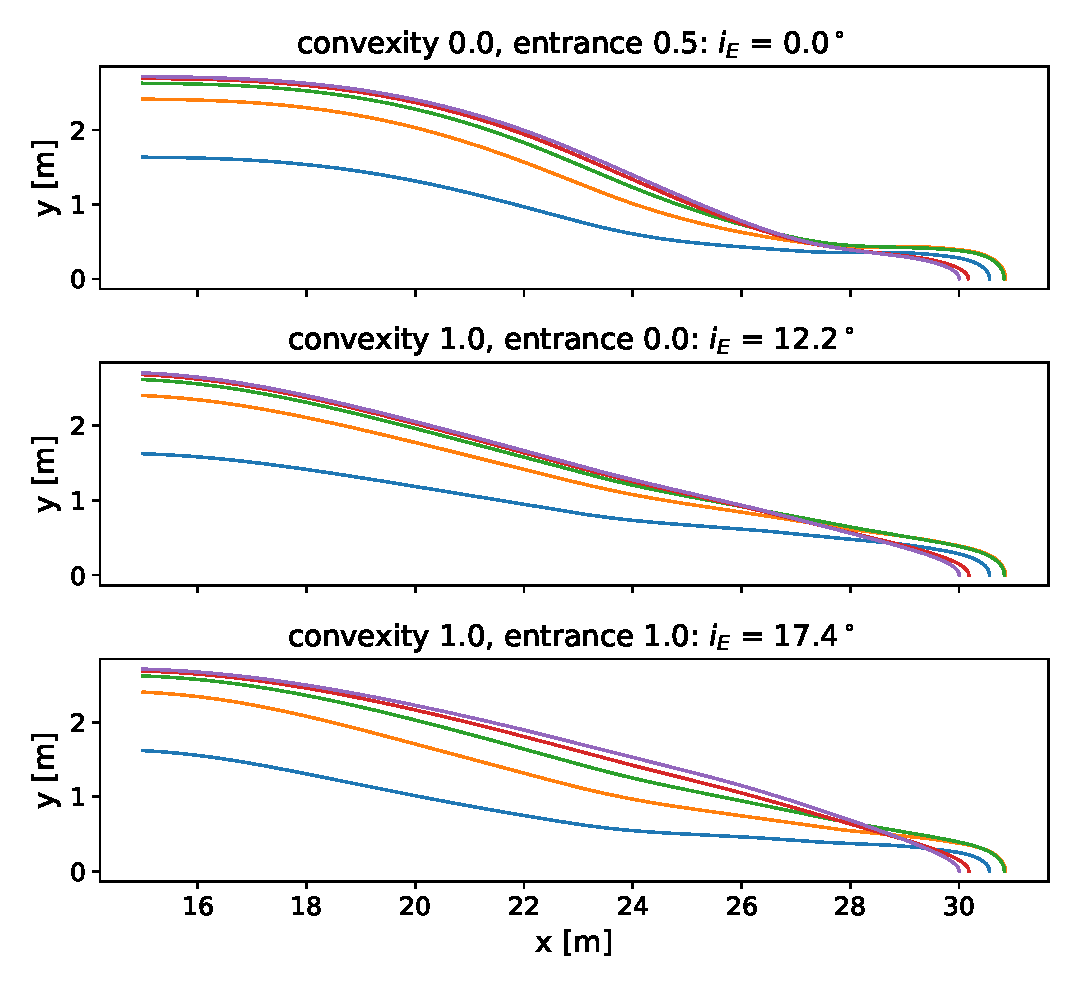
\includegraphics[width=0.75\textwidth]{figures/bow.pdf}
\caption{Effect of \cmd{bow\_convexity} and \cmd{entrance\_angle} on the forebody waterlines.}
\end{figure}

\subsection*{Fixed datum}
\label{sec:fixed}
\begin{longtable}{L{3.0cm}L{12.3cm}}
\toprule
Name & Meaning \\ \midrule
\cmd{volume} & displaced volume of the complete hull (bulb, skeg and stem rounding included) at the
design waterline [m$^3$]. It is matched exactly: with $L$, $C_P$ and $C_M$ given it fixes the
product $B\,T$, which \cmd{beam\_rel} splits into beam and draft. Realistic proportions exist
only if, approximately, $0.0062\,L^3 \le \nabla \le 0.0143\,L^3$ (e.g. 167--386\,m$^3$ at
$L = 30$\,m); the exact limits depend on $C_P$ and $C_M$, and a combination outside them is
reported by \cmd{chk\_proportions} \\
\bottomrule
\end{longtable}

\paragraph{Notes on the relative parameters.}
\begin{itemize}
\item \cmd{entrance\_angle}: the reachable range is narrow when \cmd{bow\_convexity} is low, and
  zero for a fully concave bow. The actual angle and its range are written to
  \cmd{hull\_hydro.dat} (\cmd{entrance\_angle\_deg}, \cmd{\_min\_deg}, \cmd{\_max\_deg}).
\item \cmd{bow\_fullness}: the solved midship position and the fore/aft prismatics are reported
  (\cmd{x\_max}, \cmd{Cp\_fwd\_bare}, \cmd{Cp\_aft\_bare}).
\item \cmd{C\_BB} is matched exactly when the hull itself is narrower than $B_B$ at the forward
  perpendicular; otherwise the bulb keeps a minimum amplitude and the effective value is
  reported (\cmd{C\_BB\_target}, \cmd{C\_BB\_eff}).
\end{itemize}

%=====================================================================
\section{Output files}
\subsection{PLOT3D grid}
ASCII, one block, \cmd{ni nj 1}, then all $x$, all $y$, all $z$ (index $i$ fastest), with
$i$ from bow to transom and $j$ from deck to keel. With \cmd{--nurbs-fit approx} (default) the
points lie on the analytic surface. With \cmd{interp} they are the control points of the
interpolating B-spline.

\subsection{B-spline file}
Four lines, readable list-directed in Fortran:
\begin{lstlisting}
p_u p_v                  ! degrees (u = index i, v = index j)
n_u n_v                  ! number of control points (= ni nj)
n_u + p_u + 1 knots in u
n_v + p_v + 1 knots in v
\end{lstlisting}
The control points are those of the PLOT3D file, in the same order. Weights are unitary.

\subsection{STEP file}
AP214 (ISO~10303-21). By default it is a closed solid (\cmd{MANIFOLD\_SOLID\_BREP}) with six
faces:
\begin{itemize}
\item the hull, one B-spline face per side;
\item the deck, one face per side, ruled from the deck edge to the centreplane;
\item the transom, one plane per side, bounded by the transom line and two segments to the
  centreplane at deck height.
\end{itemize}
\cmd{--step-half} writes the starboard faces only, and \cmd{--step-open} the hull faces only.

\subsection{Hydrostatics: \cmd{hull\_hydro.dat}}
One \cmd{value = name} per line, at the design waterline, for the complete hull (bulb, skeg and
stem included) unless stated otherwise.
\begin{longtable}{L{3.0cm}L{12.3cm}}
\toprule
Group & Keys \\ \midrule
Basic & \cmd{volume}, \cmd{displacement}, \cmd{LCB} (m from transom), \cmd{LCB\_frac\_L},
\cmd{LWL}, \cmd{BWL}, \cmd{Awp}, \cmd{LCF}, \cmd{S\_wet}, \cmd{A\_transom}, \cmd{T\_transom},
\cmd{T\_max}, \cmd{Cb}, \cmd{H\_dwl}, \cmd{B\_max}, \cmd{L\_over\_B\_max}, \cmd{H\_transom},
\cmd{volume\_target}, \cmd{volume\_error}, \cmd{B}, \cmd{L\_over\_B}, \cmd{B\_over\_T} \\
Form & \cmd{Cp}, \cmd{Cm}, \cmd{Cwp}, \cmd{LCB\_mid\_frac}, \cmd{Cp\_minus\_input},
\cmd{LCB\_minus\_input}, \cmd{A\_T\_over\_A\_M} \\
Stability & \cmd{KB}, \cmd{BM\_T}, \cmd{BM\_L}, \cmd{KM\_T}, \cmd{I\_T}, \cmd{I\_L},
\cmd{TPC} [t/cm], \cmd{MCT\_1cm} [t\,m/cm] \\
Ratios & \cmd{vol\_over\_01L3} ($\nabla/(0.1L)^3$), \cmd{L\_over\_vol13} ($L/\nabla^{1/3}$) \\
Design (bare hull) & \cmd{Cp\_bare}, \cmd{LCB\_bare\_mid\_frac}, \cmd{Cp\_aft\_bare},
\cmd{Cp\_fwd\_bare}, \cmd{x\_max}, \cmd{L\_pmb\_eff}, \cmd{deadrise\_mid\_deg}, \cmd{c\_bow},
\cmd{entrance\_angle\_deg} (+ \cmd{\_min}, \cmd{\_max}), \cmd{entrance\_half\_angle\_deg} (measured),
\cmd{wl\_inflections\_fwd} \\
Bulb (Kracht) & \cmd{L\_PR}, \cmd{Z\_B}, \cmd{H\_B}, \cmd{b\_bulb}, \cmd{C\_BB\_target},
\cmd{B\_B}, \cmd{C\_BB\_eff}, \cmd{A\_MS}, \cmd{A\_BT}, \cmd{A\_BL}, \cmd{V\_PR}, \cmd{C\_ABT},
\cmd{C\_ABL}, \cmd{C\_VPR} \\
Checks & \cmd{chk\_*} (1 = passed) and \cmd{feasible} (1 = all passed): finite and non-folding surface, waterline beam within $B/2$, bulb below the waterline, bulb breadth on target, volume closure, monotone run waterlines, forebody prismatic $\ge 0.55$, volume on target, realistic $L/B$ and $B/T$ \\
B-spline fit & \cmd{nurbs\_dev\_max}, \cmd{nurbs\_dev\_mean} (distance from the surface points) \\
\bottomrule
\end{longtable}

\subsection{Hydrostatic curves}
With \cmd{--hydro-curves FILE}, a table with one row per waterline in \cmd{--drafts}:
$z_{wl}$, volume, displacement, LCB, KB, LCF, $A_{wp}$, $BM_T$, $BM_L$, $KM_T$, TPC, MCT,
$S_{wet}$, $C_B$, $C_{WP}$.

%=====================================================================
\section{Troubleshooting}
\begin{description}
\item[\cmd{missing parameters / unknown parameters}] the parameter file does not contain exactly the
  33 shape parameters and the fixed \cmd{volume} of Section~\ref{sec:params} (names are checked;
  order does not matter).
\item[\cmd{variant NOT VALID}] look at the \cmd{chk\_*} keys in \cmd{hull\_hydro.dat}. Within
  the bounds of Section~\ref{sec:params} this is not expected; outside them it can happen.
\item[\cmd{Cp\_minus\_input}, \cmd{LCB\_minus\_input} not zero] expected when
  \cmd{bulb\_implicit} $<1$ (the bulb adds volume). With \cmd{bulb\_implicit} $=1$ they are only
  non-zero in extreme corners, where the compensated bare hull is not reachable.
\item[Run time] about 5\,s per hull; the section table is computed once per process.
\end{description}

\begin{thebibliography}{9}
\bibitem{kracht1978}
A.~M. Kracht, \emph{Design of bulbous bows}, Transactions of the Society of Naval Architects
and Marine Engineers (SNAME), vol.~86, pp.~197--217, 1978.
\end{thebibliography}

\end{document}
